%% We use `subfiles' package
\documentclass[preamble.tex]{subfiles}
\begin{document}

\clearpage

\chapter{Loop representation: The Loop Language}
\label{ch:Loops}

\LiveFusion at the top level is a library of high level array combinators. Most of these conceptually represent a loop. Indeed, the user of the library can reason about the individual combinators as loops and consider the result of each to be an array.

However, when running the user's program, we are aiming to perform the required operations in as few loops as possible\footnote{This may increase register pressure. However, unless register spilling poses a problem in the future we favour the decreased memory traffic which is attained by array fusion.}. \todo{We have discussed the conditions for fusible combinators in Section ... In general, however...} Subject to certain restrictions, two combinators in \LiveFusion are fusible when the output array \*produced* by one combinator is \*consumed* as input by another combinator one element at a time from beginning to end.

In the \LiveFusion AST discussed in the previous chapter, this relationship is usually seen between a child node (the producer) and its parent node (the consumer). This is not true for \*random access* combinators like @backpermute@ which we discuss separately\todo{in Section }.

\todo{How do we know whether two combinators can be fused?}Intuitively, two combinators can be fused whenever one could write a loop by hand which would give the same final result for the same input as the two separate loops would.
%We need a way to programmatically determine whether a given pair of combinators can be replace with a semantically equivalent loop.

%The focus of this chapter is to establish the requirements for fusible combinators and define a loop representation to which such fusible combinators can be mapped.
The focus of this chapter is to establish a common loop representation to which fusible combinators can be mapped.

In the following sections we will look more closely at what a loop really is and then present the core of our fusion optimisation.


\clearpage

\section{Anatomy of a loop}
\label{sec:anatomy}

Despite the purely functional, combinatorial interface to the library, looking at a loop in a procedural way is the approach I have opted for in the middle layer of the system. It is represented by the \Loop language.\iloop

The loops \LiveFusion generates can be viewed as similar to those one might write in an Assembly language. It uses labelled basic blocks and has explicit control flow using @goto@ statements\footnote{The formal grammar of the \Loop language is introduced later in the chapter. It is presented in Figure \ref{fig:Loop-grammar} on page \pageref{fig:Loop-grammar}}.

However, as we will see later, the loops are more structured than those in \C and other procedural languages. As such I urge the reader to think of them as being high-level and treat the explicit control flow as implementation details.

%The downside, however, is that our loop relies on @goto@-like statements whose use is almost always considered bad practice in modern software engineering.

Without further delaying the discussion of the matter we will now look at the structure of a typical @for@ loop in a language like \C in an attempt to shape our own loop structure.


\subsection{Structure of a \code{for} loop}

Consider the following fragment of a \C program that creates a new array @ys@, by applying some function @f@ to those elements of array @xs@ that satisfy some predicate function @p@ (in \Haskell this could be expressed as @ys = filter p $ map f $ xs@):

\begin{ccode}[numbers=left, label=lst:filterMapC]
double *ys = malloc(len * sizeof(double)); // result array
int j = 0;                                 // output index
for(int i = 0; i < len; i++) {
    if(p (xs[i])) {
        ys[j] = f (xs[i]);
        j++;
    }
}
ys = realloc(ys, j * sizeof(double));
\end{ccode}

A @for@ loop in \C has four sections:

\begin{enumerate}
\halfspacing
\item \*initialisation* section (@i = 0@),
\item \*guard* section (@i < len@),
\item the main \*body* (@if ... @), and finally
\item the \*update* section (@i++@).
\end{enumerate}

Compared to free-formed @while@ loops which only have a @guard@ and a @body@, the @for@ loops are already much more structured.

However, as we see next, further structural elements could be introduced which will ultimately assist us when composing loops from array combinators.


\subsubsection{Initialisation}

The very first observation to make is that both the result array @ys@ and the output index @j@ were declared and initialised outside the @for@ loop.

In pursuit of a more structured and composable approach to looping all statements that are executed \*once* before the loop begins are placed in the \[init] basic block of the loop.

The initialisation code corresponds to the following in the \Loop language:

\begin{loopcode}
init:
  let len = arrayLength xs
  let ys = newArray len
  let i = 0
  let j = 0
  goto guard
\end{loopcode}


\subsubsection{Guard}

The @guard@ section of a @for@ loop corresponds to the \[guard] block in the \Loop language. It can contain arbitrary statements but usually contains at least one @unless@ statement:

\begin{loopcode}[%
  literate={_xs}{{\sub{xs}}}2,%
]
guard:
  unless i < len | done
  goto body_xs
\end{loopcode}

The @unless@ \*statement* transfers the control to a different block if the specified condition is \*false* (to \[done] in this case, the finaliser block discussed later). Otherwise the control stays in the current block, which in this case results in entering the loop's body.


\subsubsection{Update}

We defer presenting the \Loop language's equivalent of the @update@ section until after the structure of loop bodies is discussed shortly.


\subsubsection{Finalisation}

In the general case the @filter@ results in a shorter array than its input. Hence, after the @for@ loop finishes, the resulting array is \texttt{realloc}'ated to free the unused memory (in practice the array is unlikely to be copied).

This is one of the use cases for what is called the \[done] block of the loop:\todo{As we will see later it is not only useful for trimming and returning the final array but also for scheduling other loops such as in @append@ combinator.}.

\begin{loopcode}
done:
  let result = sliceArray ys j   -- resize to length j
  return result
\end{loopcode}

As seen from the code, every loop has a result which it returns explicitly.


\subsection{``Dissecting loop bodies''}
\label{sec:dissecting-bodies}

We will now attempt to categorise the types of operations that all belong to the bodies of conventional @for@ and @while@ loops.

We continue using example presented on page \pageref{lst:filterMapC} as reference. In particular, the @body@ of the @for@ loop contained the following statements:

\begin{ccode}[numbers=left, firstnumber=4,]
if(p (xs[i])) {
    ys[j] = f (xs[i]);
    j++;
}
\end{ccode}



\subsubsection{Isolating combinators}

Line 5 of the @for@ loop, the statement @ys[j] = f (xs[i])@, is actually performing three operations:
\begin{enumerate}
\halfspacing
\item \*reading* an element from array @xs@,
\item \*producing* a new element by applying function @f@, and
\item \*writing* the new element into array @ys@.
\end{enumerate}

Recall, however, that we are trying to devise a loop representation for an application of fusion. When several combinators are fused into a single loop and produce no intermediate\iintermediate arrays, such reading and writing only happens at the beginning and at the end of a combinator pipeline\ipipe.

Hence we want to separate the notion of \*producing* a new element from the fact that it came from a physical array or just another computation. Likewise, we should not be concerned with how the new element is going to be consumed. It may or may not be written into a new array. It may or may not be used by a consuming combinator. However, it should not be up to an individual combinator to decide.

Each combinator in the pipeline is responsible to only take care of its own processing. In particular each combinator fills in its own \[body], \[yield] and \[bottom] basic blocks which we discuss next.



\subsubsection{Computing a new element in the \[body]}

As discussed previously, each combinator fills in a number of blocks with statements specific to it. For now we will only focus on the \[body] blocks produced:

\begin{loopcode}[%
  literate=
    {_xs}{{\sub{xs}}}2
    {_filt}{{\sub{filt}}}2
    {_map}{{\sub{map}}}3
]
body_xs:
  let x = readArray xs i

body_filt:
  unless (p x) | bottom_filt

body_map:
  let y = f x
\end{loopcode}

The reading of @xs@ array is treated as a separate combinator and results in a @readArray@ statement. The \[body] of the @filter@ is a conditional jump if the predicate @p@ is not satisfied. Lastly, the \[body] of @map@ is the application of function @f@ to element @x@ and binding it to a fresh variable @y@.

We know however, that if @filter@ produces and element, then so does @map@. We say that @filter@ and @map@ produces elements at the same \term{rate}. Thus we can \*merge* the respective blocks of the two:

\begin{loopcode}[%
  literate=
    {_xs}{{\sub{xs}}}2
    {_filt}{{\sub{filt}}}2
    {_map}{{\sub{map}}}3
]
body_xs:
  let x = readArray xs i

body_filt/_map:
  unless (p x) | bottom_filt
  let y = f x
\end{loopcode}

It was mentioned that each combinator also introduces \[yield] and \[bottom] blocks.

The complete \Loop generated for @ys = map f $ filter p $ xs@ as well as its control flow graph (CFG)\icfg are shown on Figure~\ref{fig:MapFilterLoop}. In addition to \[init], \[guard], \[body] and \[done] blocks it also contains \[yield] and \[bottom] block with the required control flow. A step-by-step explanation of these spans the following four sections.


\subsubsection{Yielding produced elements}

The \Loop language attempts to be precise as to where the element is produced and where it is consumed. More concretely, the \[yield] block of the loop is only ever entered if an element has been produced in the current iteration.

\begin{bluebox}
The \[body] block contains the code that is concerned with producing an element, however an element is known to have been produced only if the control reaches the \[yield] block.
\end{bluebox}

Every \[body] block on the listing is accompanied by the \[yield] block. The combinator reading the @xs@ array in \[body$_{xs}$] produces an element @x@ at every iteration, hence the corresponding \[yield$_{xs}$] block is entered unconditionally.

On the other hand, the @filter@ (and the subsequent @map@) may skip an element hence the possibility possibility of bypassing \[yield$_{filt/map}$] block.

This allows us to make assumptions about the behaviour of a loop without knowing what the loop is doing internally.


\subsubsection{Writing an element into result array}

The separation of \[yield] and \[body] has allowed for a finer grained loop structure.

In particular, if the result of a combinator has to be materialised into the physical array (as in the the case of @map@ in our example), the @writeArray@ statement needs to be inserted into \[yield$_{map}$]:

\begin{hscode}
writeArray ys j y  -- write element y into array ys at index j
\end{hscode}


\subsubsection{Updating index}

The \[yield] block also provides a convenient place to update the index variable.

In our example the loop contains two \*rates*\irate:
\begin{itemize}
\item one at which the elements are read from the source array,
\item and one at which the elements of @filter@ and @map@ are produced
\end{itemize}

With the current loop structure, updating both @i@ and @j@ index is a matter of placing an increment statement in the right \[yield] block:

\begin{loopcode}[%
  literate=
    {_xs}{{\sub{xs}}}2
    {_filt}{{\sub{filt}}}2
    {_map}{{\sub{map}}}3
]
yield_xs:
  i := i + 1
  goto body_filt

yield_filt/_map:
  writeArray ys j y
  j := j + 1
  goto bottom_map
\end{loopcode}

As seen in the code above \Loop language supports destructive updates through using @assignment@ (@:=@).

This introduction of the index update is uniform for all \*rates* that may be present in the loop. This is in contrast to the @for@ loop originally presented on page \pageref{lst:filterMapC} where @i++@ was part of @update@ section, while @j++@ was inside the @for@ loop's body. 


\subsubsection{Ending the iteration}

When the iteration has finished the last block that is entered \*unconditionally* (for each rate) is \[bottom]. In the given examples the two \[bottom] blocks simply transfer the control to the beginning of the next iteration, the \[guard]. However, in more sophisticated loops, e.g. @append@ combinator\todo{\ref{sec:append}}, the \[bottom] blocks may serve other purposes.


%%%%%%%%%%%%%%%%%%%%%%%%%%%%%%%%%%%%%%%%%%%%%%%%%%%%%%%%%%%%%%%%%%%%%%%%%%%%%%%
%% Final Loop for mapFilter example.
\begin{figure}

\begin{subfigure}{.6\textwidth}
\begin{loopcode}[%
  literate=
    {_xs}{{\sub{xs}}}2
    {_filt}{{\sub{filt}}}2
    {_map}{{\sub{map}}}3
]
init:
  let len = arrayLength xs
  let ys = newArray len
  let i = 0
  let j = 0
  goto guard

guard:
  unless i < len | done
  goto body_xs

body_xs:
  let x = readArray xs i
  goto yield_xs:

yield_xs:
  i := i + 1
  goto body_filt



body_filt/_map:
  unless (p x) | bottom_filt
  let y = f x
  goto yield_map:

yield_filt/_map:
  writeArray ys j y
  j := j + 1
  goto bottom_map

bottom_filt/_map:
  goto bottom_xs



bottom_xs:
  goto guard

done:
  let result = sliceArray ys j
  return result
\end{loopcode}
\end{subfigure}%
%
\begin{subfigure}[right]{.4\textwidth}
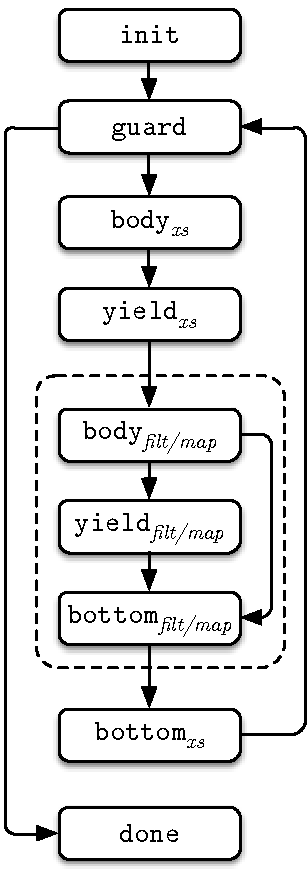
\includegraphics[center,scale=\omniscale]{img/CFG-MapFilter}
\end{subfigure}

\caption{Internal \Loop language representation for \code{ys = map f $ filter p $ xs} (left) and the corresponding CFG (right).}
\label{fig:MapFilterLoop}
\end{figure}


\subsection{Summary of Loop structure}
\label{sec:anatomy-summary}

In summary the common loop structure to be used throughout this chapter\footnote{At least until segmented combinators are introduced.\todo{in ref}} is comprised of the following 6 loop sections, represented by basic blocks in the \Loop language:\iblock
\begin{enumerate}
\item \[init] block is the main entry into the loop and contains statements which need to execute only once for the whole loop. New array allocation, index and length variable initialisation all belong here.
\item \[guard] block performs looping condition tests before every iteration of the loop.
\item \[body] block contains all statements concerned with reading arrays and computing elements. This block is \*rate*-specific and there is a new \[body] block for every distinct rate in the loop.
\item \[yield] block for a particular rate is entered only if a \*new element* has been produced by the \[body] block of the same rate in the current iteration. It is not entered if the loop's logic has skipped to the next iteration without producing an element (e.g. in @filter@ combinator). This is the place to update the loop index as well as \*write* the produced element in the resulting array if required.
\item \[bottom] block is entered unconditionally at the end of every iteration whether of not an element has been produced. Uses beyond going back up to the beginning of the next iteration will be seen later in this chapter.
\item \[done] block performs any remaining operations after the loop has finished. In particular it returns the final result from the loop. Unlike the loops in the majority of procedural languages the @return@ of values \*from a loop* is explicit in the \Loop language.
\end{enumerate}

Figure~\ref{fig:CFG-basic} shows the default control flow between these sections.

\begin{figure}[h!]
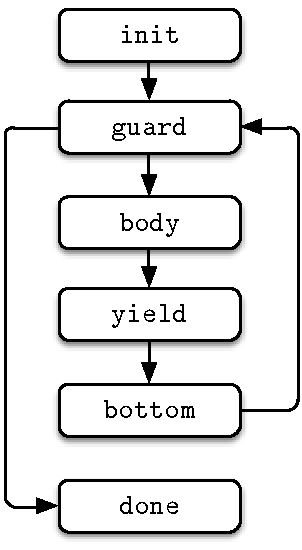
\includegraphics[center,scale=\omniscale]{img/CFG-basic}
\caption{Default control flow between basic blocks in the \Loop language.}
\label{fig:CFG-basic}
\end{figure}



\clearpage

\section{The \Loop language more formally}
\label{sec:The-Loop-language}
\iloop

So far we have used the following features of the \Loop language:
\begin{enumerate}
\halfspacing
\item New variable binding (@i = 0@)
\item Variable assignment (@i := i + 1@)
\item Explicit control transfer (@goto body@)
\item Conditional control transfer (@unless i < len | done@)
\item Returning values from loop (@return ys'@)
\item A number of built-in array primitives: (@newArray@, @readArray@, @writeArray@, @arrayLength@ and @sliceArray@).
\end{enumerate}

All of the above are \*statements*, which are grouped into labelled \*basic blocks*.\iblock

The grammar of the \Loop language is presented formally in Figure~\ref{fig:Loop-grammar}. The syntax seen in the examples throughout this thesis is the same as used by the pretty printer for the language and it faithfully\footnote{I have taken the liberty of rewriting operators in infix notation and omitting explicit literal conversions such as \code{fromInteger 1}.} reproduces the internal representation of \Loop programs. 

\begin{figure}[htpb]
\subfile{loop-grammar}
\caption{\label{fig:Loop-grammar}Grammar of \Loop language.}
\end{figure}
\todo{Put the footnotetext on the same page where the grammar ends up}
\footnotetext{For improved readability the unique integers are replaced with meaningful names in the code listings. \*(Footnote for listing \ref{fig:Loop-grammar})*}

If the grammar is studied more carefully one would note that one basic block may have multiple associated labels. We have seen a use case for this when we merged \[body], \[yield] and \[bottom] basic blocks of @filter@ and @map@ combinators (Figure~\ref{fig:MapFilterLoop}). Such merged blocks can be referenced by either label. For example, \[bottom\sub{filt/map}] was being referenced both by \[bottom\sub{filt}] and \[bottom\sub{map}].

It should also be noted that each label and variable in the language is postfixed with a unique value which has so far been omitted from the listings. However, \[body\sub{xs}] is an example of such label identification. At the implementation level these values are unique integers. However, for improved readability they are replaced with combinator names and other meaningful identifiers.

Being a flexible assembly-style language, the \Loop language is not limited by the basic block structure discussed in Section~\ref{sec:anatomy} and summarised in Section~\ref{sec:anatomy-summary}. However, as seen in the rest of this chapter this structure has proven to be a useful common base for many types of arrays combinators. Thus we assume this to be the common pattern of using the \Loop language.

Semantically, the \Loop language does not presume a fixed order of evaluating @let@ bound variables. However, all statements affecting control flow (@goto@, @unless@, @if@) are executed in the order they appear in the block.

% Lastly, the new value of assigned variables ($\coleq$) is not available until the next block the control is transferred to. This is an implementation side-effect of the \*liveness analysis* pass (Section~\ref{sec:Liveness-analysis}) which however is helpful in implementing fused loops.


\clearpage

\section{Fused loops generation}
\label{sec:loop-generation}

In the previous section we have seen the first example of the \Loop EDSL which computed a @filter@ of an array followed by a @map@. We have also identified five main \*sections* of a loop, represented by \*basic blocks* in the \Loop language: \[init], \[guard], \[body], \[yield], \[bottom] and \[done].

We shall revisit the example from the previous section and introduce the process by which a \Loop is generated.

This time we extend the example with specific functions passed to @map@ and @filter@ combinators. The function @toPercentages@ shown on Figure~\ref{fig:toPercentages} (left) converts an array of fractions to their percentage equivalents, filtering out those below $0.01$ (or $1\%$).

\begin{figure}
\begin{subfigure}{.66\textwidth}
\begin{hscode}
toPercentages :: Array Double -> Array Double
toPercentages fractions
  = let significant = filter (>=. 0.01) fractions
        percents    = map (* 100) significant
    in  percents
\end{hscode}
\end{subfigure}%
%
%\begin{subfigure}{.3\textwidth}
%  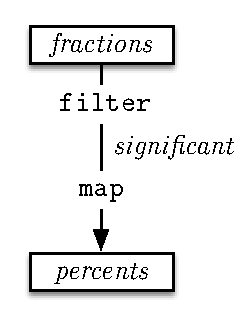
\includegraphics[height=12em]{img/toPercentages-flow}
%\end{subfigure}
%
\begin{subfigure}{.34\textwidth}
  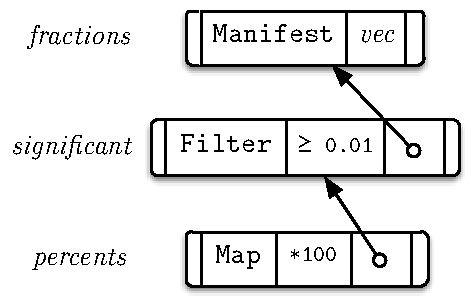
\includegraphics[scale=\omniscale]{img/AST-toPercentages}
\end{subfigure}
\caption{\code{toPercentages} function (left) and its \LiveFusion AST (right).}
\label{fig:toPercentages}
\end{figure}



\subsection{Start with an AST}

The @toPercentages@ function internally uses a pipeline of two combinators: the output array of @filter@ (called @significant@) becomes the input array of @map@. Recalling that @Array Double@ is the type synonym for @AST (Vector Double)@, each combinator constructs a node in an AST representing a \*delayed array computation*.

It is not known statically if the input array, @fractions@, is computed by a pipeline of combinators or whether it is a @Manifest@ array stored in memory. Likewise, it is not known before runtime if the resulting @percents@ array is consumed by another combinator and the pipeline of delayed operation will continue to grow after @toPercentages@ function returns.

For the purposes of illustrating a complete running example we will assume that the @toPercentages@ function is called with a @Manifest@ array as argument and the result is immediately \*forced* to be computed (e.g. to be written out to a file or to be consumed in a random access fashion).

In this case the AST shown on Figure~\ref{fig:toPercentages} (right) is constructed and \*forced* to a @Manifest@ array at the runtime of the program:

\begin{hscode}[mathescape]
-- AST that may be a result of a call to toPercentages
ast :: AST (Vector Double)
ast = force
    $\dol$ Map (* 100)
    $\dol$ Filter (>=. 0.01)
    $\dol$ Manifest vec

-- LiveFusion library functions
force :: Elt a => AST (Vector a) -> AST (Vector a)
force = Manifest . evalAST

evalAST :: AST a -> a
evalAST = $...\ compile\ AST\ and\ compute\ result ...$
\end{hscode}

The three fusible combinators represented by @Manifest@, @Filter@ and @Map@ AST nodes are followed by the call to an evaluator, which processes them individually as shown next.
% After sharing recovery each AST node (or rather ASG node) is assigned a unique value


\subsection{Generate loops for individual combinators}
\label{sec:individual-loops}

In order to generate the \Loop language code for an AST of combinators, the evaluator first processes combinators individually. For each combinator it populates the sections of the loop that were identified in Section~\ref{sec:anatomy}. It does so by inserting new statements into the appropriate basic blocks of a loop template.

\subfile{lst-toPercentages-loops}

The left of Figure~\ref{fig:toPercentages-loops} shows the loops generated for the individual combinators. It is implicitly referenced in the following discussion.

All variables and labels introduced by a particular combinator are given a unique identifier. In listings these are: \*mfst* (short for \*Manifest*), \*map* or \*filt*.

Internally however, the library uses unique integers to distinguish between similarly named variables and labels belonging to different combinators (e.g. @body_2@ and @elt_3@). This not only avoids variable name clashes, but as we discuss next, enables communication among combinators through naming conventions.



\subsubsection{Iterate over a \code{Manifest} array}
\label{sec:manifest}

Recalling that the @Manifest@ combinator is the only combinator in the pipeline that holds a reference to the physical array, its loop does nothing more than to read the array @arr@\sub{mfst} element by element.

It is worth noting that the array is not @let@-bound in any of the blocks. This is due to the fact that the array is an \*argument* to the loop and is passed from the running program when the computation is finally ready to be performed (code generation and loading are discussed in Chapter~\ref{ch:Code-Generation}).

The combinator introduces a length variable @len@\sub{mfst} which it binds in loop initialisation block @init@\sub{mfst}.

The result of array read is placed in @elt@\sub{mfst} variable.

Notably, the combinator does not bind the index variable @ix@\sub{mfst} itself but assumes that it's present in scope. The insertion of appropriate index variables is done after the complete loop is analysed and all \*rates* are established.\todo{as discussed in ref}


\subsubsection{Filter}

In the loop representing @filter@ code all bound variables and label names are identified by \*filt*.

As discussed previously in Section~\ref{sec:Scalar-language} it is essential for performance that the user functions parametrising combinators be inlined in the generated code. In case of the @filter@ the predicate function $(\geq 0.01)$ has been inlined as the predicate expression to the @unless@ statement.

While the length of output array of @filter@ may be different from the length of input, the \*upper bound* on the length is the same as that of the previous combinator. This is expressed by binding the length variable @len@\sub{filt} to @len@\sub{mfst} of the @Manifest@ combinator.

Similarly, the resulting element @elt@\sub{filt} is bound to be @elt@\sub{mfst} -- the output of @Manifest@ in the same iteration of the loop.



\subsubsection{Map}

Populating the loop with @map@-specific statements is straight-forward.

Since the length of the output of @map@ is always the same as the length of input, the @len@\sub{map} variable is simply rebound. This also means that @Manifest@, @filter@ and @map@ share the same \*upper bound* on the length of their output arrays. %This means that @Manifest@ combinator uses one index, while both @filter@ and @map@ are using another. This supports the \*rate*-changing\irate nature of @filter@.

To compute @elt@\sub{map} for the current iteration, we only need to know @elt@\sub{filt}, that is the element produced by the previous combinator \*in the current iteration*.

Again, the user specified function $(* 100)$ is inlined to facilitate generation of fast code.


\subsubsection{Physical array creation}

For the @toPercentages@ example we said the pipeline of combinators will be forced to a @Manifest@ array immediately after the @map@.

The statements required to allocate, populate, slice and return the new array are self-explanatory.

It is worthy of note that the design decision to transfer control to \[yield] basic block only when an element is produced has made it very easy to introduce the array write.



\subsection{Rates and looping}
\label{sec:rates}\irate

Multiple times throughout this thesis, the concept of \term{rates} has been mentioned.

\begin{bluebox}
\term{Rate} is a property of a combinator within a combinator graph. If two combinators are statically known to produce arrays of the same length, they are said to have the same \term{rate}.
\end{bluebox}

For example, all three @map@s in @map h . map g . map f@ are known to share the same rate since their inputs and outputs will be of the same length.

For the same reason the @filter@ and the subsequent @map@ of the @toPercentages@ example share the same rate since they both produce same-length arrays. As such, they are assigned a single index variable @ix@\sub{filt} (Figure~\ref{fig:toPercentages-loops}).

However, the @filter@ combinator has earlier been identified as \*rate-changing*. In particular we treat @filter@ as a combinator producing elements at a \term{subrate} of the previous combinators. In the @toPercentages@ example, the @filter@ was preceded by @Manifest@, which receives it's own separate index variable @ix@\sub{mfst}.

\begin{bluebox}
If the rates of combinators are equal they share one index variable and their corresponding blocks can be merged together.

If a combinator runs at a \*subrate* of another combinator then it has its own \[body], \[yield] and \[bottom] blocks since it may not produce an element at every iteration.
\end{bluebox}

Rate equality and subrate relationship are not the only possible relationships between two combinators. We will introduce other relationships when we discuss segmented combinators.\todo{in Section~ref}



\subsection{Naming conventions}
\label{sec:naming-conventions}

As seen from the loop code generated for the individual combinators in the @toPercentages@ example, the \Loop language uses a set of \*naming conventions* to facilitate communication between consecutive combinators in a pipeline. In particular the following are always true for a combinator with identifier \*id*:

\begin{itemize}
\halfspacing
\item Variable @elt@\sub{id} contains the value of produced element at every iteration
\item Variable @len@\sub{id} contains the upper bound on the length of the output array
\item Variable @ix@\sub{id} contains the index of the element being produced.
\end{itemize}

Binding @elt@\sub{id} and @len@\sub{id} in every combinator ensures that this information is \*propagated* upwards through the pipeline of combinators. In particular, the @filter@ only required to know the \*id* of @Manifest@ combinator below it to infer these variables.

\begin{bluebox}
By design the combinators know their own unique identifiers and the unique identifiers of the combinators they are referencing and nothing else.
\end{bluebox}



\subsection{Merging loops}

We have given the \Loop language representations for @Manifest@, @map@ and @filter@ combinators as well as the code that writes out physical arrays.

In order a create a succinct loop, these individual loops are merged into one loop.
%In order a create one succinct loop, these individual loops are merged into one loop as they are being created. Each combinator has access to the loop composed by all of the combinators below it. For example, when fusing the @map@ the cumulative loop of both @filter@ and @Manifest@ is available for it to be merged with.

For combinators as simple as @map@ and @filter@ merging loops means to simply merge the statements of the corresponding blocks blocks in no particular order.

As seen from the final loop on Figure~\ref{fig:toPercentages-loops} (right), not only the block statement lists have been merged together, but also the block labels: each block can now be identified by any of the three identifiers (\*mfst*, \*filt*, \*map*).

This is done in order to support fusing complex ASTs with many shared nodes. The benefit of this may appear much clearer when we introduce nested combinators\todo{in Section}.
\todo{Elaborate.}


\subsubsection{Managing label sets with \name{AliasMap}}

In order to achieve the flexibility of having multiple labels associated with the same block I have implemented a new type of associations @Map@ called \name{AliasMap}.

It offers a familiar interface (Listing~\ref{lst:AliasMap-interface}) similar to that of \Haskell's @Data.Map@. The difference is that it allows for a \*set* of keys to be associated with one value. In addition to the usual functions found in @Data.Map@ one can query the map using \*synonyms*. That is, a value can be retrieved from the map given any key associated with that value.

The notion of \*key synonyms* is used throughout \name{AliasMap} interface which greatly facilitates managing and merging loops where blocks are associated with multiple labels.

\lstinputlisting[style=haskell, float, caption={\name{AliasMap} interface (partial). \code{Ord k} constraints omitted for brevity.}, label=lst:AliasMap-interface]{listings/AliasMap-interface.hs}


\clearpage
\section{More on \texttt{goto}s}

While the use of @goto@s is considered bad practice in modern software engineering I note several reasons for using them in the \Loop intermediate language:

\begin{itemize}
  \item It is completely hidden from the library user.

  Given a well behaving \Loop code generator the produced code will always be valid if the user program is valid.

  This is akin to using @unsafePerformIO@ and the like within the library internals for performance reasons. They can lead to bad code but with careful use give very noticeable advantages to purely functional programs.


  \item The \Loop language was designed with a pluggable backend in mind.

  It was assumed that assembly-like \Loop language would be easier to connect with any backend.

  Specifically in the \Haskell backend, @goto@ statements are translated to tail-recursive function calls.

  An \LLVM backend is also planned. \LLVM uses a very similar notions of \*basic blocks*.


  \item The @goto@ based design was the most flexible and the easiest to implement.

  Nonetheless, this does not prevent the \Loop language from being extended to support a safer programming model.
\end{itemize}




\clearpage
\section{Flat array combinators}

\todo{Intro to the section. Say it's going to be brief. \ref{fig:CFG-basic}}


\subsection{Reductions}

We have already looked at how the indices maintain the state of the loop between iterations. Although it is probably the most obvious state a loop has, it is not the only one. Perhaps the most prominent standard list combinators that pass partial results to recursive calls as accumulators are @fold@s and @scan@s. \LiveFusion also offers these combinators.

In practice, binding and using accumulator variables like this in the \Loop language is straight-forward and is no different from binding and using index variables. They are both treated as mutable variables in the \Loop language.

Suppose, we wanted to translate @scan (*) 0 xs@ to a loop. As discussed previously in Section~\ref{sec:naming-conventions} on naming conventions the generation of loop blocks for @scan@ proceeds in assumption that variables @len@\sub{xs} and @elt@\sub{xs} are in scope.

The following is the portion of the loop generated for @scan@ combinator:

\begin{loopcode}[%
  literate=
    {_1}{{\sub{scan}}}3
    {_3}{{\sub{xs}}}1,
]
init_1/_3:
  let len_1 = len_3
  let z_1 = 1
  let acc_1 = z_1

body_1/_3:
  let elt_1 = acc_1

bottom_1/_3:
  acc_1 := acc_1 * elt_3
\end{loopcode}

Generating loop code for @fold@ is very similar except no element @elt@\sub{fold} is produced in each iteration and the final result is stored in @acc@\sub{fold}.


\subsection{Zipping}
\label{sec:zipping}

So far the combinator pipelines we have looked at had a list like structure. Each combinator would consume exactly one array and produce another. However, for many programs this is not sufficient. Many combinators take multiple arrays as input.

In general there is no constraint on how a combinator would consume each of those arrays. Some combinators (e.g. @backpermute@) require that one of the argument arrays can be accessed randomly. Combinators like @append@ and @interleave@ consume arrays independently and not at the same time.

However, there are combinators like @zipWith@$N$ which consume $N$ arrays in lock step.

A call to @zipWith (*) xs ys@ element-wise multiplies @xs@ and @ys@. Those two arrays may internally be pipelines of combinators. It results in the following \Loop code:

\begin{loopcode}[%
  literate=
    {_1}{{\sub{zip}}}2
    {_2}{{\sub{xs}}}1
    {_3}{{\sub{ys}}}1,
]
init_1/_2/_3:
  let len_1 = len_2

body_1/_2/_3:
  let elt_1 = elt_2 * elt_3
\end{loopcode}

The code is similar to that of @map@ (Figure~\ref{fig:toPercentages-loops}). In fact @zipWith@$N$ combinators can be viewed as generalised @map@s.

There are two problems with @zipWith@$N$ family of combinators:

\begin{enumerate}
\item The lengths of @xs@ and @ys@ may be different.
\item The loops for @xs@ and @ys@ may not produce elements in every iteration.
\end{enumerate}

Appendix~\ref{ch:zipping-problems} considers both problems in turn, offering potential fusion strategies for each. While these may be legitimate cases to consider in a general purpose fusion framework, they do not appear in the vectorised \name{Data Parallel Haskell} code. Since \DPH is currently the primary target for the application of \LiveFusion, the fusion of these cases is left as future work.



\clearpage

\section{Random access combinators}

\subsection{Backpermute}

\subsection{Index}



\clearpage

\section{Array generators: Enumeration and Replication}

\subsection{Segmented array combinators}

Two types

\subsection{Segmented scan}

\subsection{Segmented fold}

\subsection{Segmented replicate}



\clearpage

\section{Interleaved loops}

\subsection{Append}

\subsection{Segmented append}


\IfNotCompilingAll{\bibliography{bib}}

\end{document}
